\chapter{点缺陷}
   % 本部分的内容来自于其他文档,请参考:空位与缺陷.pdf文件。
    在早期的晶体X射线衍射强度的研究中,就已经发现几近完整的晶体中存在有缺陷。
    早在1914年,达尔文提出了图像不很明确的嵌镶组织,用来解释实际晶体的X射线
    衍射和理想的完整晶体的差异嵌镶组织的概念长期为人使用,但是没有进一步的发
    展,直到位错理论确立后,才清楚了嵌镶组织的确切图像。在20年代,Frenkel为
    了解释例子晶体导电的实验研究,提出了晶体的点缺陷理论。40年代初,塞兹和
    亨丁顿研究了金属中点缺陷的一些基本性质,目的是为了阐明扩散的机制。50年代后
    由于原子能反应堆技术的进展,高能粒子对固体的辐照效应引起了人们的重视,又
    推动了对于晶体中的点缺陷作全面而深入的研究。

    \section{分类和定义}
        点缺陷\index{点缺陷}是指原子尺度的缺陷。其特征是所有方向的尺寸都很小,也被称为零
        维缺陷。包括空位\index{点缺陷!空位}、杂质\index{点缺陷!杂质}或溶质原子\index{点缺陷!溶质原子}、
        间隙原子\index{点缺陷!间隙原子}以及它们组成的复杂缺陷,比如空位对\index{点缺陷!空位对}
        或空位集团\index{点缺陷!空位集团}等。

        \subsection{空位}
            如果在晶体中抽取在正常点阵座位上的一个原子就造成了点阵的空位。
            也可以说,晶格的节点上缺了一个原子,这个地方称为晶格空位。

            经典的空位图像是简单的:在晶体结构中抽取一个原子后,周围的原子基本
            保留在原有的位置上,留下一个很明确的空位。如果周围原子朝向空位
            作较大的松弛,或者崩塌到空位里面,这就形成一种弥散的空位或者十几个原子构成的
            松弛集团,类似与局部的熔区,有人称之为松弛群\index{点缺陷!空位!松弛群}。
            这两种不同的空位图像还很难通过直接的观察来证实,但是晶体的皂泡筏模型对解决这个问题提供了一些线索。
            在皂泡筏模型的\cite{book:1106816}中,一般温度下,空位是很明确的,符合经典的
            图像,只有在接近熔点的温度,才和松弛群的图像有些类似。

            原子离开格点后,有两种存在的方式,一是离开格点到达晶体表面,二是从点阵位置到达间隙位置,
            这时这个原子就变成一个溶质原子,也称为间隙原子\index{点缺陷!空位!间隙原子}。

        \subsection{溶质原子}
            溶质原子主要包括间隙原子或置换固溶原子,其中处于间隙的位置是间隙原子,
            处在基体点阵中间隙处的同类原子是自间隙原子,处于间隙位置的异类原子成为杂质型间隙原子。

            处于点阵位置,置换式或替代式的外来原子取代本身原子,处于晶格节点上的异类原子
            称为置换原子。

            间隙原子的情况要比空位复杂一些,以面心立方的晶体为例,面心立方晶体中
            的间隙位置,最大的间隙位置是八面体型的$[\frac{1}{2},\frac{1}{2},\frac{1}{2}]$,
            如果间隙位置处于八面体位置的正中心,将周围的原子稍加挤开,这就是第一种可能的组态,
            所产生的畸变具有球面对称性,如\autoref{面心立方中的两种间隙}所示;
            第二种可能的组态为间隙原子沿 $\langle 100 \rangle$方向偏离了一些,点阵上的一个近邻原子也偏离
            平衡位置,形成一对原子的哑铃式间隙组态.所产生的畸变具有四方对称性,如\autoref{哑铃型间隙原子}所示;
            另一种是挤列型组态,在密排方向有,$n+1$个原子占据了$n$个原子的位置,如\autoref{挤列型间隙原子}所示。
            \begin{figure}[ht]
                \centering
                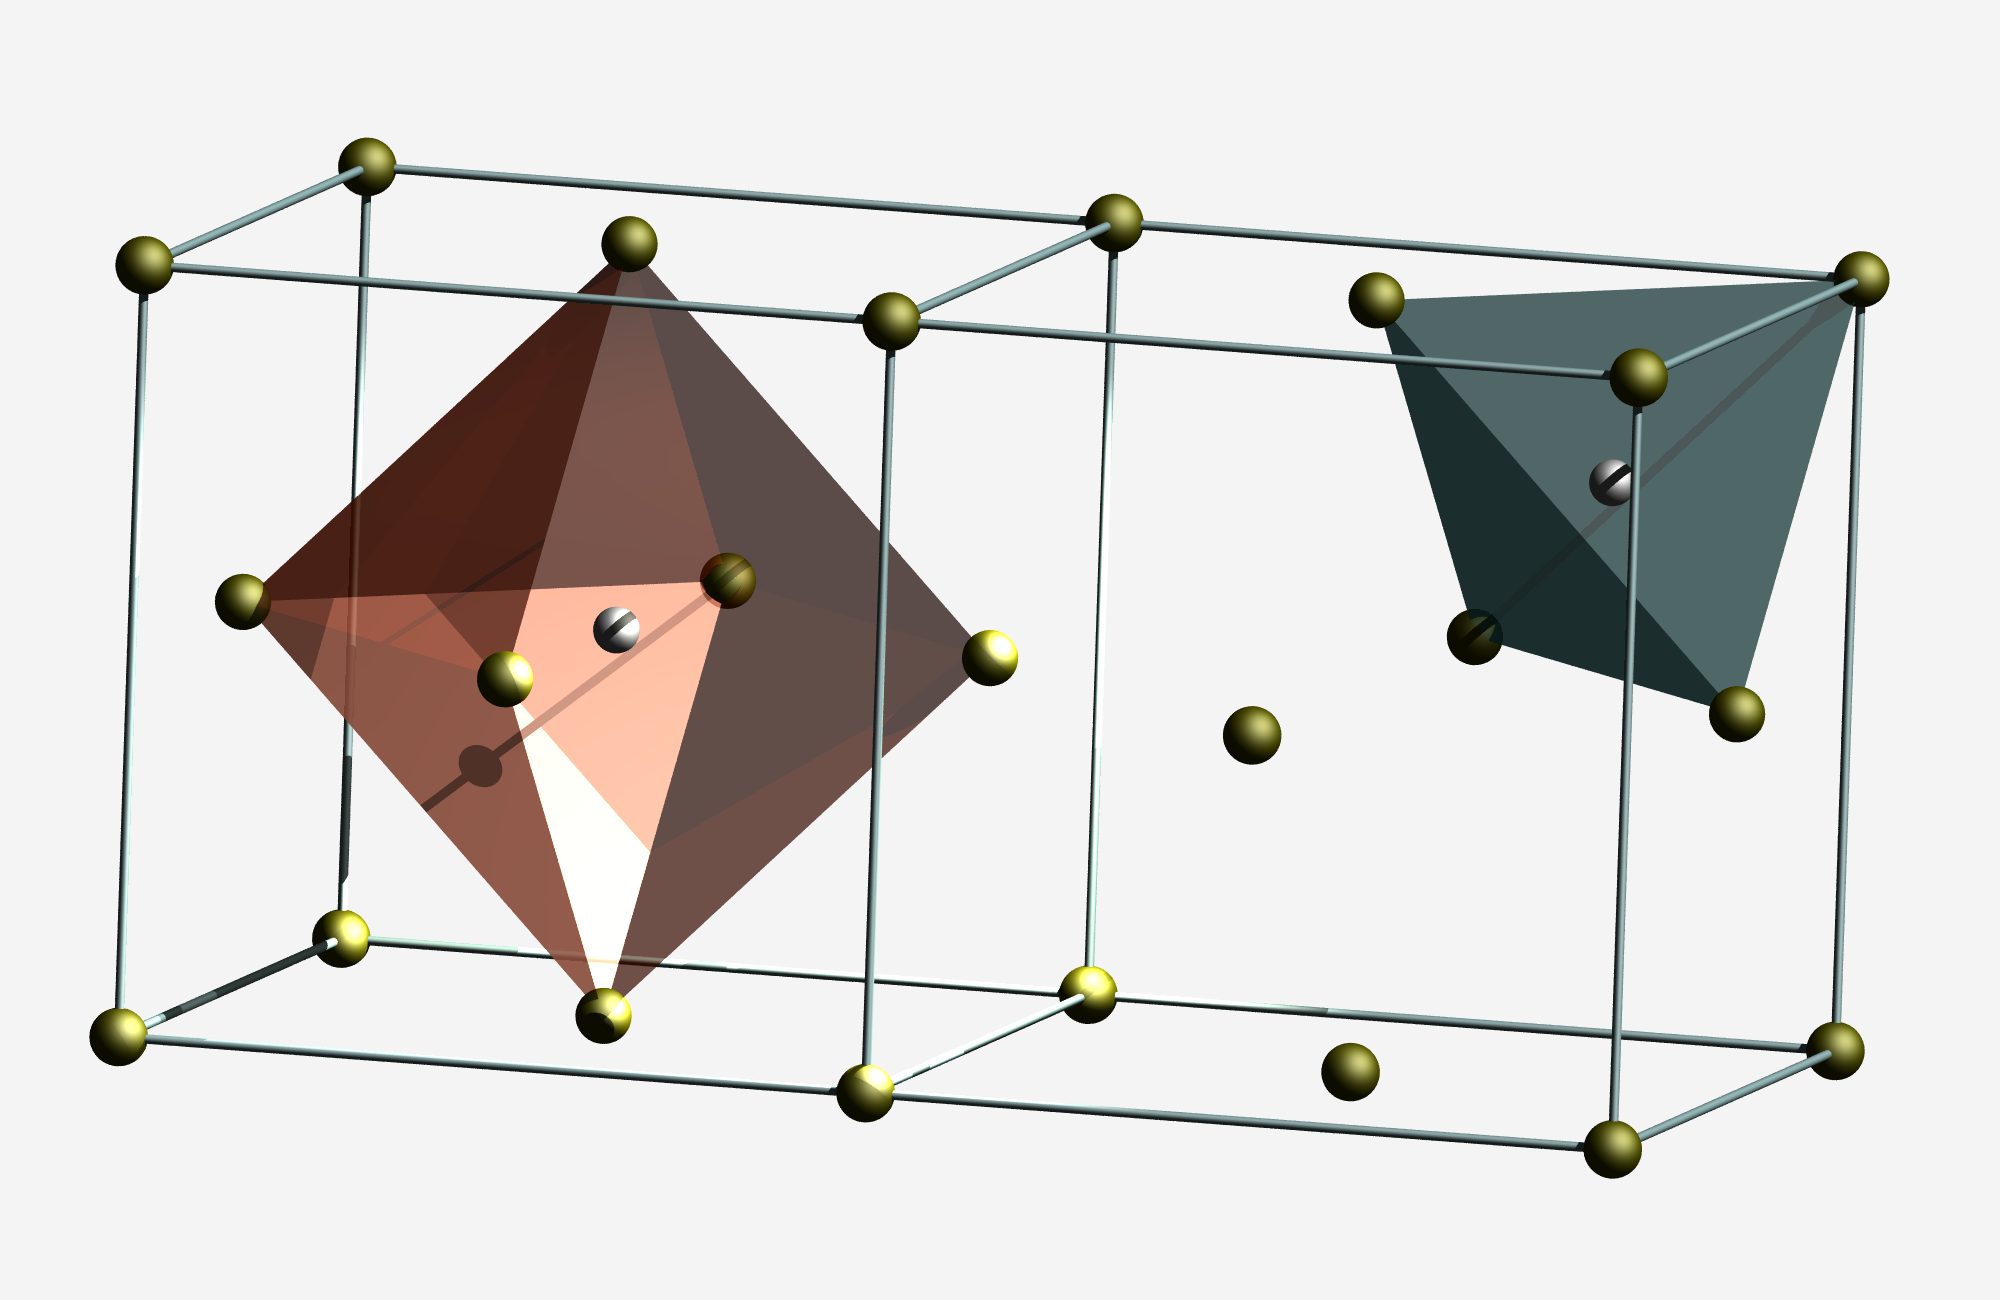
\includegraphics[width=0.7\textwidth]{fig/polyhedra_in_fcc.png}
                \caption{面心立方中的两种间隙。}
                \label{面心立方中的两种间隙}
            \end{figure}
            \begin{figure}[ht]
                \centering
                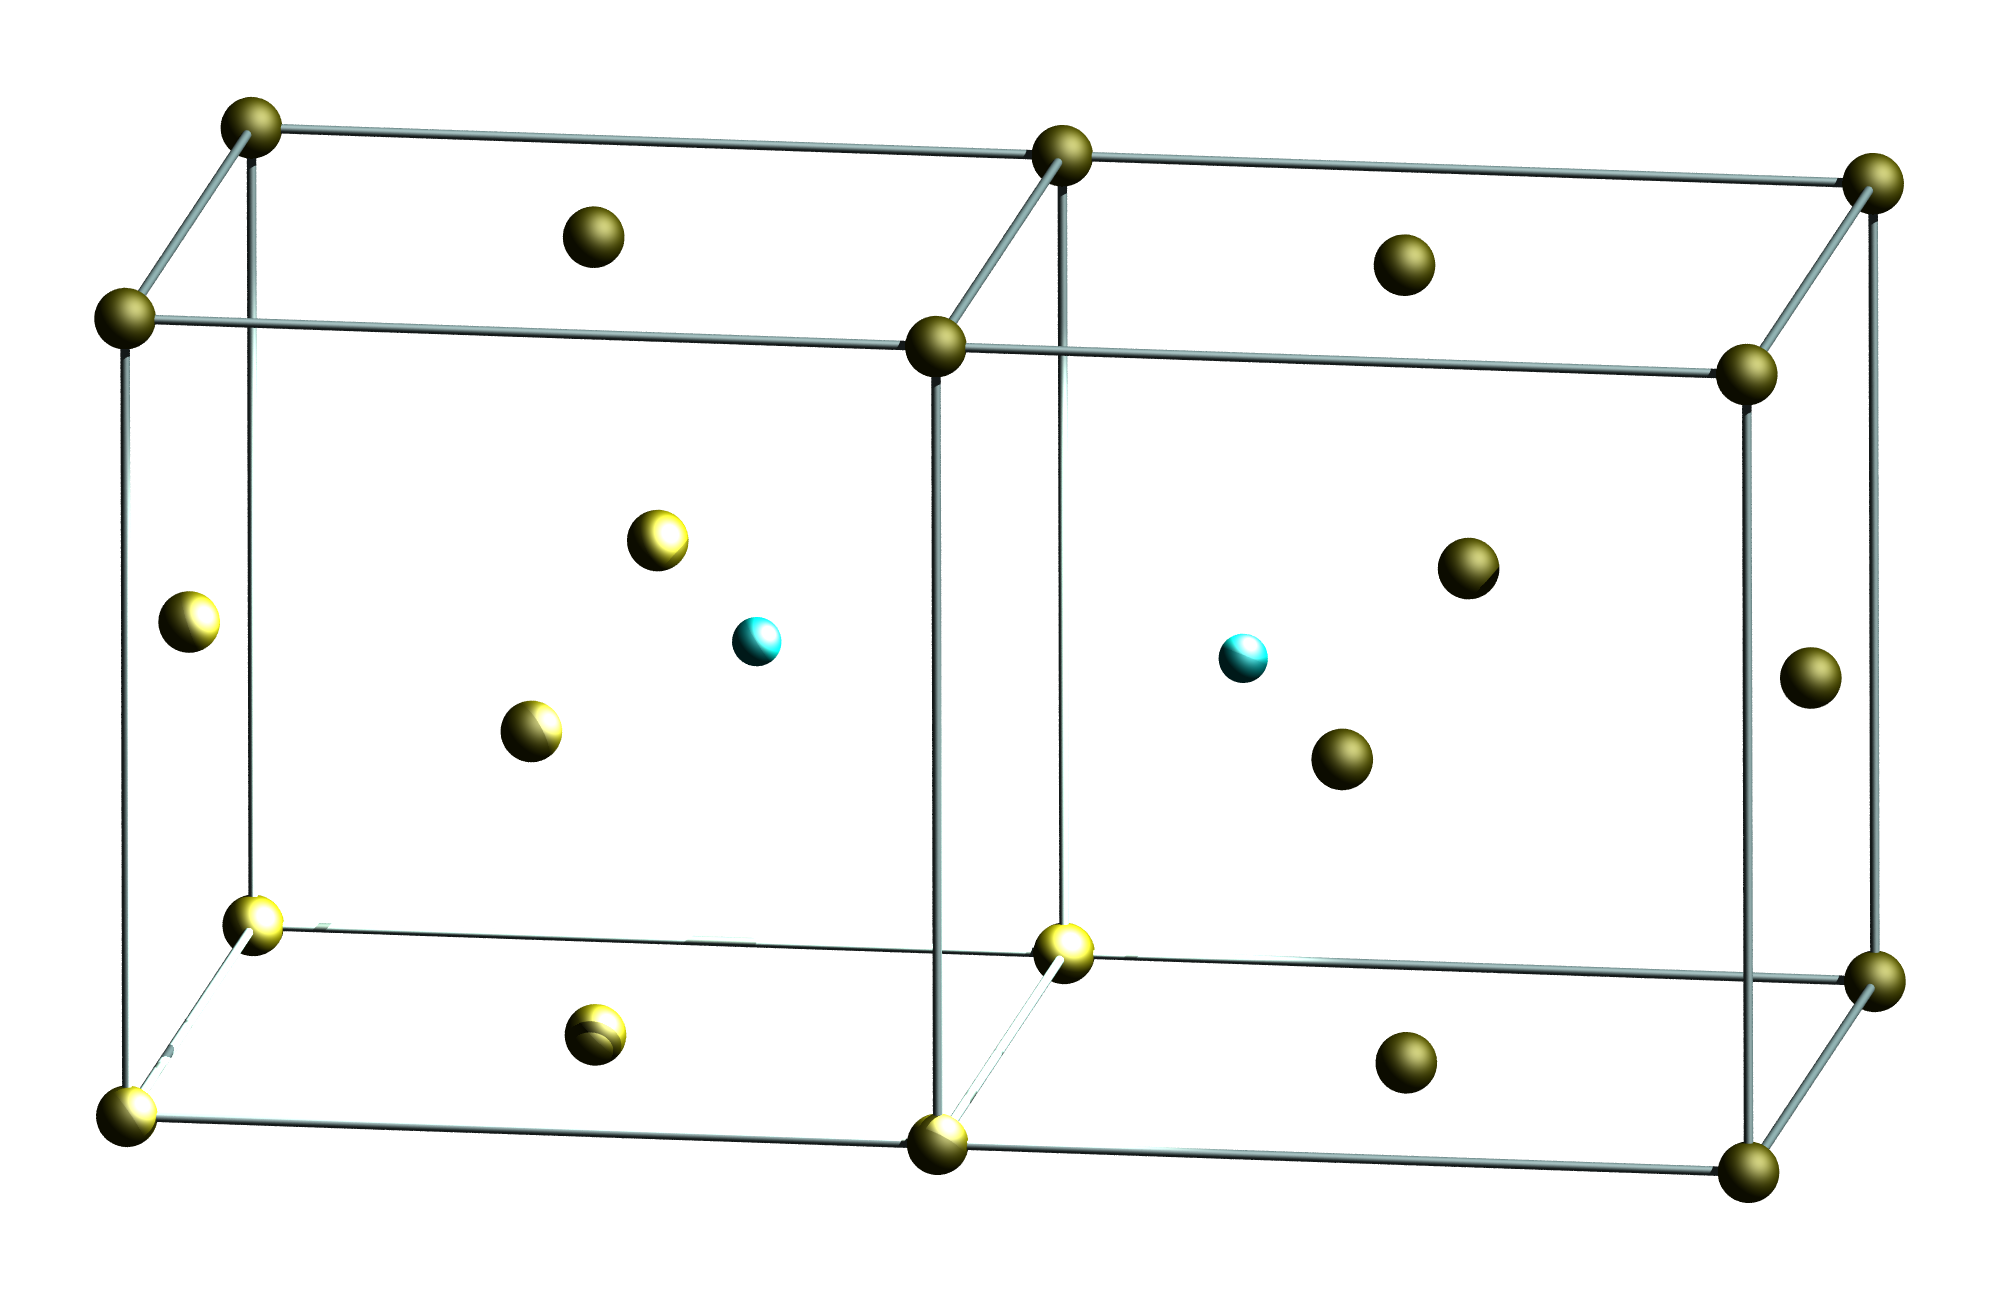
\includegraphics[width=0.7\textwidth]{fig/interstitial_in_fcc.png}
                \caption{哑铃型间隙原子。}
                \label{哑铃型间隙原子}
            \end{figure}
            \begin{figure}[ht]
                \centering
                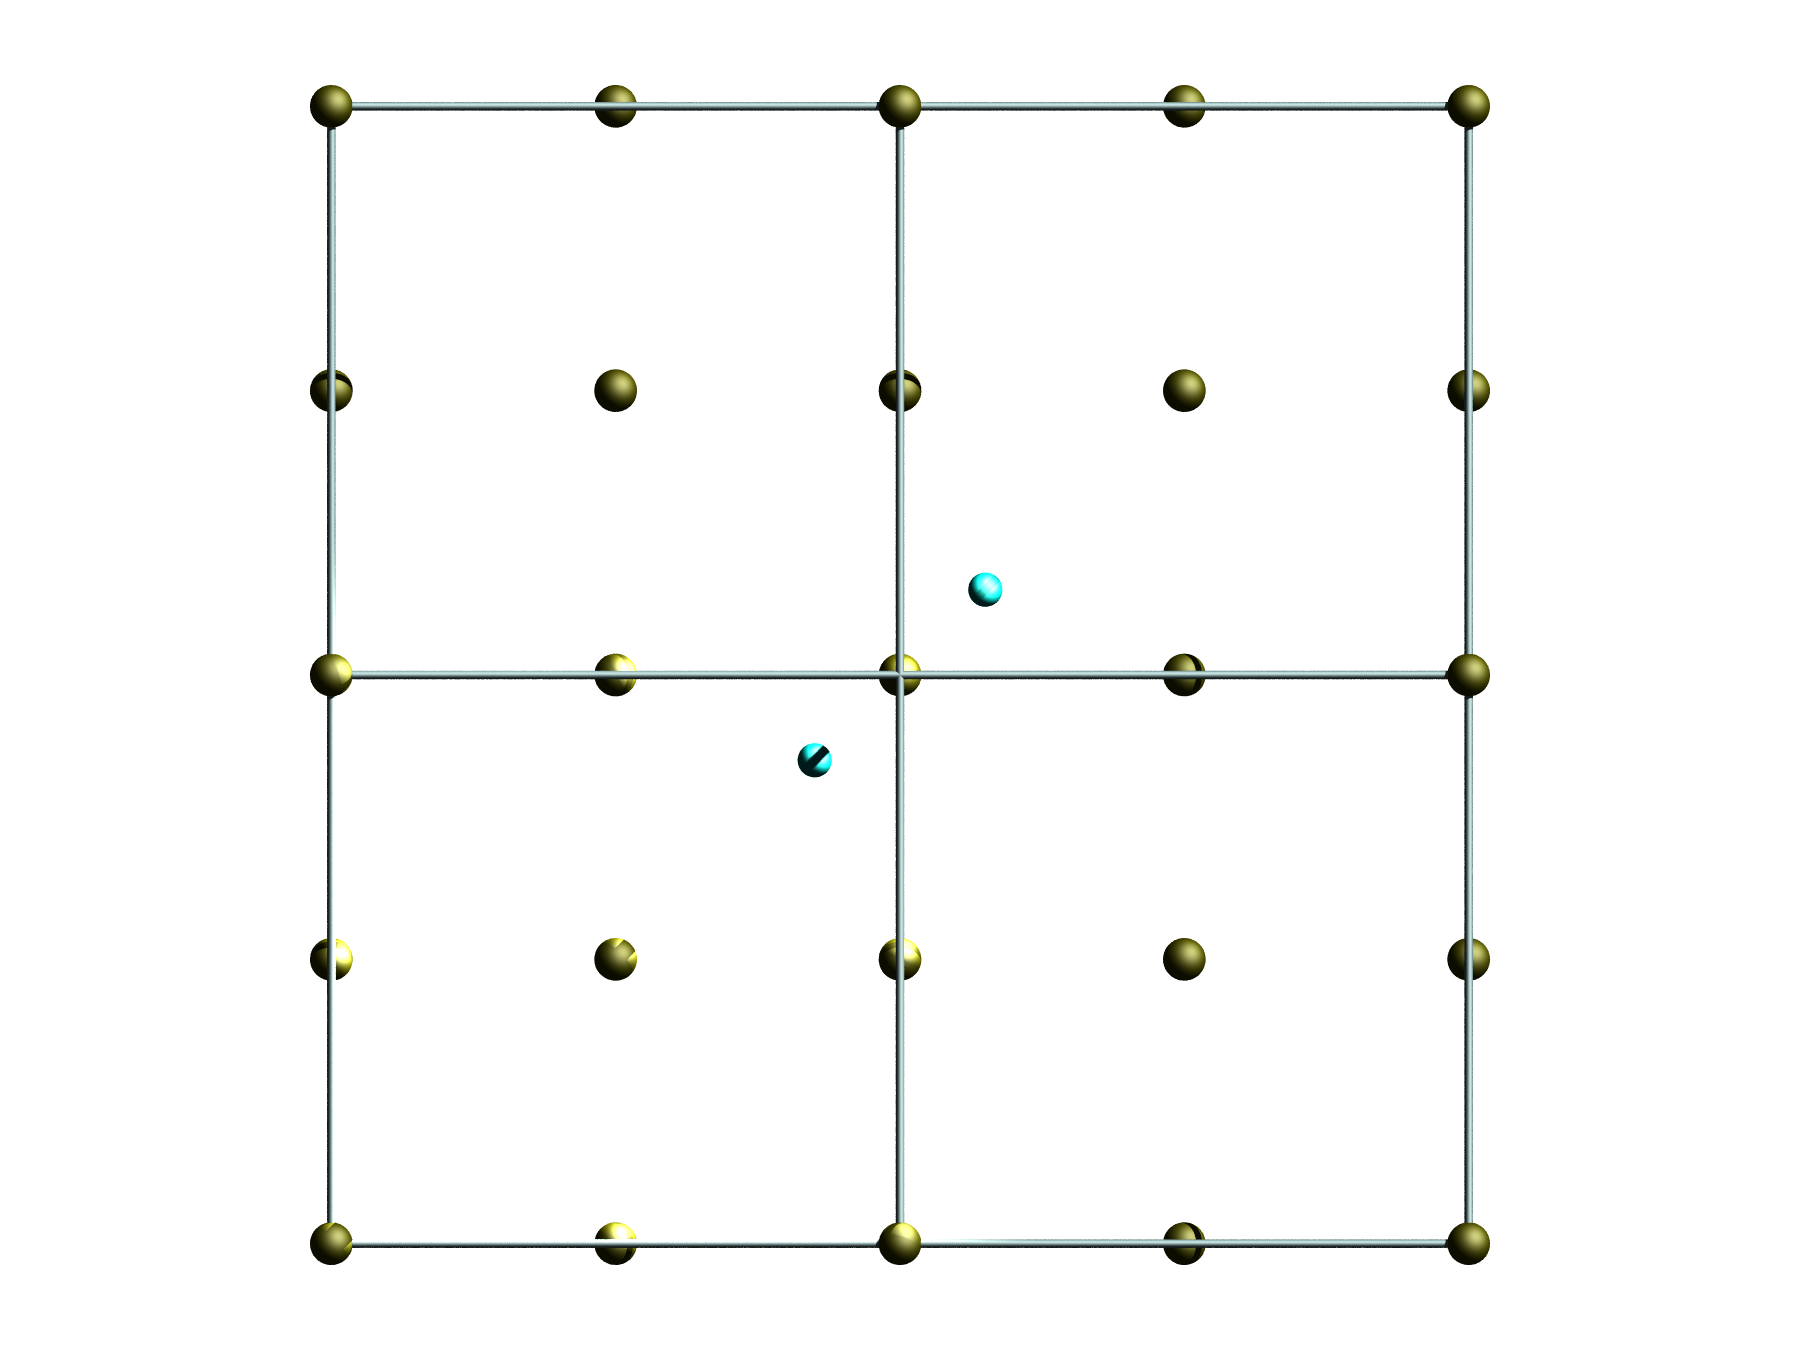
\includegraphics[width=0.5\textwidth]{fig/interstitial_in_fcc_3.png}
                \caption{挤列型间隙原子。}
                \label{挤列型间隙原子}
            \end{figure}
            
            只有对这些不同组态的间隙原子的能量进行细致的理论计算后,方能判定那一个组态具有
            最低的能量,因而是平衡组态.理论计算结果表明哑铃组态能量最低,这已为实验观察所证实。

            间隙原子引起的畸变(包括异类原子和自间隙原子):总引起扩大(膨胀),周围有一个压缩区;
            外来原子比基体原子大,则膨胀,形成压缩区;比基体原子小,则形成张力区。

        \subsection{复合点缺陷}
            由于缺陷之间的相互作用,容易形成复合缺陷,如空位对,空位集团等。在这里主要关注热缺陷,
            也就是由于晶体中的原子或离子的热运动而造成的缺陷,从几何图形上看与属于点缺陷,热缺陷
            的数量与温度有关,温度越过,造成缺陷的机会也越多。晶体中热缺陷有两种形态,分别是Schotty
            曲线和Frenkel缺陷。

            首先关注Schotty缺陷,由于热运动,晶体中阳离子及阴离子脱离平衡位置,
            跑到晶体表面或晶界位置上,构成一层新的截面,而产生阳离子空位及阴离子空位,
            不过这些阳离子空位与阴离子空位是符合晶体化学计量比的。比如在\ce{MgO}晶体中
            形成\ce{Mg^{2+}}和\ce{O^{2-}}的空位数相等;而在\ce{TiO2}中,每形成一个
            \ce{Ti^{4+}}离子空位,就形成两个\ce{O^{2-}}。肖脱基缺陷实际产生过程是:
            由于靠近表面层的离子热运动到新的晶面后产生空位,然后,
            内部邻近的离子再进入这个空位,这样逐步进行而造成缺陷。

            对于Frenkel缺陷,形成过程是一种离子脱离平衡位置挤入晶体的间隙位置中去,形成所
            谓间隙(或称填隙)离子,而原来位置形成了阳离子或阴离子空位。这种缺陷的特点是
            间隙离子和空位是成对出现的。弗仑克尔缺陷除与温度有关外,与晶体本身结构也有
            很大关系,若晶体中间隙位置较大,则易形成弗仑克尔缺陷。如\ce{AgBr}比\ce{NaCl}
            易形成这种缺陷。
    \section{点缺陷的形成能}
        点缺陷定义为形成一个点缺陷所需要的能量,以空位为例,空位的形成能被定义
        为在晶体内取出一个原子放到晶体的表面上(但不改变晶体的表面能)所需要的能量。
        为了不影响晶体的表面积,去除的原子应当位于表面的台阶处。可以用类似的方式来定义
        填隙原子的形成能,也就是从晶体表面台阶上取下一个原子,挤进晶体原子间隙所需的能量。

        可以对空位的形成能进行一个简单的估计。假设晶体为面心立方结构,只考虑
        原子间最近邻的相互作用。由于面心立方晶体的配位数为12,从晶体内部取出
        一个原子应当切割12个键,而在表面结合还要再形成6个键,因此相当于一共切割了
        6个键,而且与结合能相等。然而这样的估计是非常简略的,因为金属键的特征、空位周围原子的位移
        等因素并没有被考虑在内。更为精确的计算表面,空位的形成能只为结合能的$\frac{1}{2}$到$\frac{1}{4}$。
        但是空位形成能和结合能之间有密切关系是符号实验事实的,结合能越大,熔点也越高,
        空位的形成能也越大。

        目前计算空位形成能的计算方法主要有三类:
        \begin{itemize}
            \item[1] 自由电子理论计算空位形成能;
            \item[2] 德拜温度或金属的熔点计算空位形成能;
            \item[3] 用原子对作用能计算空位形成能。
        \end{itemize}

        在计算中要注意几个问题:空位引起的畸变较小,形成能
        计算中,电子能占主要地位,畸变能其修正作用;间隙原子的畸变能占主要位置,电
        子能项处于次要地位;间隙原子的形成能较大,约比空位形成能大好几倍。
    
    \section{点缺陷的平衡浓度}
        \subsection{空位平衡浓度表达式}
            由于晶体中存在原子热振动,造成了原子的能量起伏,一定情况下,可以在热激活
            的作用下,原子离开正常位置,产生空位,同时产生间隙原子,同时间隙原子也可以自由
            移动,在某个瞬间可以与空位结合,从而湮灭,因此晶体中总是存在空位形成和消失的动态平衡。
            因此在热力学平衡条件下,晶体中会存在着平衡的空位浓度。

            从能量的关系来分析可以更加清楚,一方面点缺陷的存在是晶体的内能增加,但是另一
            方面,从混乱程度的增加,晶体的熵也加大。根据自由能表达式
            \begin{equation}
                F=U-TS,
            \end{equation}
            其中,$F$为自由能,$U$为内能,$T$为温度,$S$为熵,
            可以看出,一定量的点缺陷有可能使晶体的自由能下降。根据自由能极小的条件,可以求出
            热力学平衡状态下的点缺陷浓度。

            假设晶体中有$N$个原子位置,其中形成$n$个空位的排列方式为
            \begin{equation}
                \omega_c=\frac{\left( N+n \right)!}{N!n!},
            \end{equation}
            也就是体系的微观状态数,同时形成$n$个空位的形成能为$nE_f$,根据玻尔兹曼关系
            \begin{equation}
                S=k\ln{\Omega},
            \end{equation}
            $\Omega$为微观状态数,可以求得体系的组态熵
            \begin{equation}
                S=k\ln\omega_c.
            \end{equation}
            

            不存在空位的晶体的熵为零,因此空位数为$n$的熵增为
            \begin{equation}
                \Delta S_c=k\left[ \ln\frac{\left( N+n \right)!}{N!n!} -\ln1\right]=k\left[\ln (N+n) !-\ln N !-\ln n !\right]\label{n个空位晶体熵增},
            \end{equation}
            由于晶体中原子的数目原因大于1,因此可以使用\href{https://baike.baidu.com/item/%E6%96%AF%E7%89%B9%E6%9E%97%E5%85%AC%E5%BC%8F}{Stirling近似}
            \begin{equation}
                \ln{N!}\simeq N\ln N-N,
            \end{equation}
            则\autoref{n个空位晶体熵增}可以写作
            \begin{equation}
                \begin{aligned}
                    \Delta S_c&=k\left[ (N+n)\ln(N+n) -(N+n)-N\ln N+N-n\ln n+n\right]\\
                    &=k\left[ (N+n)\ln(N+n)-N\ln N-n\ln n \right].
                \end{aligned}
            \end{equation}
            另外,空位还引起振动熵增加$\Delta S_f$,此时体系的自由能表达式为
            \begin{equation}
                \begin{aligned}
                    \Delta F&=nE_f-T(\Delta S_c+\Delta S_f)\\
                    &=n(E_f-T\Delta S_f)-kT\left[ (N+n)\ln(N+n)-N\ln N-n\ln n \right],
                \end{aligned}\label{空位体系自由能变化}
            \end{equation}
            由于体系平衡时自由能为最小,因此在一定温度下达到平衡时有
            \begin{equation}
                \left( \frac{\partial \Delta F}{\partial n} \right)_T=0.
            \end{equation}
            代入\autoref{空位体系自由能变化}可得
            \begin{equation}
                \begin{aligned}
                    \left( \frac{\partial \Delta F}{\partial n} \right)_T&=\frac{\partial\left[n E_{f}-T\left(\Delta S_c+n \Delta S_{f}\right)\right]}{\partial n}\\
                    &=(E_f-T\Delta S_f)-\frac{\partial\left\{k T[(N+n) \ln (N+n)-N \ln N-n \ln n]\right\}}{\partial n}\\
                    &=\left(E_{f}-T \Delta S_{f}\right)-k T\left[\ln (N+n)+\frac{N+n}{N+n}-\ln n-\frac{n}{n}\right]\\
                    &=E_{f}-T \Delta S_{f}-k T \ln \frac{N+n}{n}\\
                    &=0.
                \end{aligned}
            \end{equation}
            由此可以解得
            \begin{equation}
                \frac{N+n}{n}=\exp\left( {\frac{E_{f}-T \Delta S_{f}}{k T}} \right),
            \end{equation}
            因此空位平衡浓度
            \begin{equation}
                c_v=\frac{n}{N}\simeq\frac{n}{n+N}=\exp{\left( (-\frac{E_f}{kT}+\frac{\Delta S_f}{k}) \right)}.
            \end{equation}
            令
            \begin{equation}
                A=\exp\left( {\frac{\Delta S_f}{k}} \right),
            \end{equation}
            空位在特定温度下的平衡浓度可以写作
            \begin{equation}
                c_v=A\exp\left( {-\frac{E_f}{kT}} \right)\label{空位平衡浓度}.
            \end{equation}
            由此也可以看出,空位是\textbf{热力学平衡缺陷}。
            
            用类似的方式可以求出间隙原子的浓度表示式.间隙原子平衡浓度为
            \begin{equation}
                c_i=q\exp\left( -\frac{E_f^i}{kT} \right),
            \end{equation}
            其中$E_f^i$为间隙原子的形成能。

            类似与化学反应,空位对与空位之间也存在平衡关系
            \begin{equation}
                \mathrm{AB}\leftrightarrow \mathrm{A}+\mathrm{B},
            \end{equation}
            假设$E_b$为空位对形成时释放的能量,则
            \begin{equation}
                E_{2f}=2E_f-E_b,
            \end{equation}
            因此空位对的平衡浓度为
            \begin{equation}
                c_{vv}=ZA^{\prime}\exp{\left( -\frac{E_{2f}}{kT} \right)}=ZA^{\prime}\exp{\left( -\frac{2E_f}{kT}-\frac{E_b}{kT} \right)},
            \end{equation}
            利用\autoref{空位平衡浓度},可得
            \begin{equation}
                \frac{c_{vv}}{c_v^2}=AZ\exp{\left( \frac{E_b}{kT}\right)}.
            \end{equation}

            由此可得,温度上升时,$c_v$以指数方式增加,则接近熔点时,$c_v$一般在$10^{-3}$到$10^{-4}$
            范围内;由于间隙原子形成能是空位形成能的3至4倍,对应的平衡浓度非常小。

            温度降低时,$c_{vv}$会增加,且结合能越大,温度越低,空位结合成双空位的趋势增加。
        
        \subsection{空位形成能的测量}
        根据前面得到的空位平衡浓度的表达式,可以很清楚看出,如果能够测得空位的
        平衡浓度随温度的变化趋势,则可很容易由这个表达式测量空位的形成能。

        实验中选取一个物理量X,其余空位浓度有一定的关系,然后测量X与温度的变化关系,
        然后得到空位浓度与温度变化趋势,同时利用空位平衡浓度的表达式\autoref{空位平衡浓度},
        就可以求出空位的形成能。实验中常用的两种方法为点阵测量法和淬火电阻法。

        点阵测量法的主要思想是,当格点上的原子离开格点形成空位时,某些原子跑到晶体表面
        上。因此晶体三维尺寸的变化不仅与空位数目有关,还与表面增加的原子数有关。而
        点阵常数得变化则只与空位的引入有关,而与表面增加的原子数没有关系。

        由于点缺陷增加,电子的散射增加,表现为电阻增加,附加电阻的大小和点缺陷
        浓度成正比,因而可用来作为点缺陷浓度的标志。从附加电阻和温度的关系可以定出
        空位的形成能.有两种不同的测量方法:
        \begin{itemize}
            \item[1] 直接在高温测量电阻对温度的曲线,曲线上的异常部分归结为空位的影响;
            \item[2] 将样品淬火,令金属迅速冷却下来,过饱和的空位就被冻结,可以保留到室温或低温.根据不同温度淬火后电阻测量的结果,也可求出空位的形成能。
        \end{itemize}

    \section{点缺陷对物理性能的影响}
        晶体中有了点缺陷,其一系列的物理性能都会受到影响。比较引人注意的是点缺
        陷对于密度及电阻的影响:
        \begin{enumerate}
            \item[1] 密度与线度,如果在点阵中取走一个原子,放到表面上去,点阵就形成一个空
                    位.如空位周围原子都不移动,则应使晶体体积$V$增加一个原子体积,而点阵常数$a$
                    保持不变.但是实际上空位周围原子会产生位移,因此$V$和$a$都有变化.理论计算的结
                    果表明,填隙原子引起的体膨胀约在1到2个原子体积,而空位的体膨胀约为0.5个原子体积;
            \item[2]  电阻 点缺陷对于传导电子产生附加的散射,引起电阻的加大.关于点缺陷的
            电阻的理论计算,一般是套用夫里德耳的合金理论,将点缺陷看为零价或一价的杂质
            的原子.但是填隙原子所引起的畸变较大,效应不易正确估计,结果的差异也较大。
        \end{enumerate}
    
    \section{点缺陷的移动}
        \subsection{空位的迁移过程}
            前面提到,晶体中存在着空位的产生,空位的迁移,空位的消失的动态平衡过
            程,因此点缺陷并不是固定于一个位置,以空位为例,空位也不是固定于一个原子坐
            位上固定不动地,而是不断地和周围原子交换位置,空位在晶体中的平衡分布是一个
            动态的平衡。因此要计算在热平衡状态下一个空位在单位时间内的跃迁次数,或称空
            位的移动频率。空位周围的近邻原子如果跃入空位,其结果就是那个原子和空位交换
            了位置,就是空位跃迁了一次。因此,空位在单位时间中的跃迁几率首先决定于空位
            的近邻原子数。即配位数$Z$。
            
            但是,空位的第一近邻原子要跃入空位还需要具备有适当
            的能量。这是由于从空位到另一个空位必须将附近的原子挤开,其中受力最大的状态则成为
            鞍点状态,此时的能量也最高。这也要求热涨落必须要提供间隙原子越过鞍点的能量。

            假设一些原子处在鞍点状态的时间足够长,我们可以把鞍点状态当做和晶体保持
            热平衡的一种组态,和空位组态和晶体处于热力学平衡那样。我们可以预料处于
            鞍点状态的原子数$n$为
            \begin{equation}
                n=N\exp\left( -\frac{\Delta G_m}{kT} \right),
            \end{equation}
            其中$N$为原子格点数,$\Delta G_m$为形成一个鞍点原子所需的Gibbs自由能,
            原子过了鞍点状态以后自由能恢复正常。$\Delta G_m$包括两部分
            \begin{equation}
                \Delta G_m=\Delta H_m-T\Delta S_m\simeq \Delta U-T\Delta S_m,                
            \end{equation}
            式中$\Delta G_m$称为激活自由能,$\Delta H_m$为激活焓,$\Delta U_m$为激活能。
            由于在通常情况下$p\Delta V$可以忽略,才可以使用上式的近似,$\Delta S_m$为原子
            到达鞍点的熵变化,$\Delta G_m$的物理意义可以认为是振动的原子A在恒温恒压下
            可逆地有原来的格点位置到鞍点位置所需要的功。
            
            因此$n/N$就是一个原子由于自由能的涨落而能够跃到鞍点的几率,用$v$表示,考虑到原子可以扩散到
            最近邻的每一个空位,因此单位时间中空位的跃迁几率为
            \begin{equation}
                \Gamma=Zv\exp{\left( -\frac{\Delta G_m}{kT} \right)},
            \end{equation}
            其中$Z$为原子配位数。
        \subsection{迁移激活能的测定}
            空位迁移激活能的测量原则主要是利用自扩散的空位机制,因此存在
            \begin{equation}
                \Delta U_m=Q-E_f,
            \end{equation}
            其中$\Delta U$为空位迁移激活能,$Q$为自扩散激活能,$E_f$为空位形成能。

            实际测量时采用分段等温退火法 通过测量电阻下降速率从而得到空位的迁移
            激活能,利用的原理是电阻下降的速率决定于空位消失速率,而空位消失的速率
            \begin{equation}
                v=\exp\left(- \frac{\Delta U_m}{kT} \right).
            \end{equation}

            具体操作步骤是。首先将样品在一个比较高的温度做长时间的保温,然后通过实
            际测量淬火到不同温度下$T_1$和$T_2$,通过保温不同的时间$t_1$和$t_2$,
            使样品电阻下降值相同,也就是
            \begin{equation}
                \left( \frac{\dif \rho}{\dif t} \right)_{T_1}\cdot t_1=\left( \frac{\dif \rho}{\dif t} \right)_{T_2}\cdot t_2,
            \end{equation}
            可以解得
            \begin{equation}
                \frac{t_1}{t_2}=\exp\left[ -\frac{\Delta U_m}{k}\cdot\left( \frac{1}{T_1}-\frac{1}{T_2} \right) \right].
            \end{equation}
            以此来计算迁移激活能。
    \section{平衡及非平衡点缺陷的产生}
        点缺陷作为一种热力学平衡缺陷,其浓度在达到热力学平衡状态时回达到一个平
        衡的数值,因此存在着点缺陷的平衡浓度的概念。但在实际中,晶体经常要经历不同
        的热历史,热力学平衡态只是一个比较特殊的状态,更多的状态确实非平衡态。例如
        淬火是金属热处理的基本方法之一,传统用来保留高温的合金相或产生亚稳的过渡相
        (如钢中的马氏体)。但认识到淬火可以保留过饱和的空位的事,对于澄清金属中空位
        的性质起很大的作用。对一些合金的淬火效应的研究表明,空位的冻结在许多传统的
        热处理过程(例如铝合金的时效)中也起很重要的作用,值得注意。因此,
        淬火作为一种产生过饱和的非平衡的点缺陷的方法被人们广泛研究。

        淬火过程中可以利用快速冷却将淬火温度下的热力学平衡空位浓度冷却到室温,从而
        得到比室温下平衡空位浓度大得多的过饱和空位浓度,很显然,这些过饱和空位属于
        非平衡空位,如果经过长时间的保温是会消除的。

        空位的产生方法就是将格点上的原子抽走,一般使用高能粒子轰击的方法。
        原子能的发展,对于金属研究提出了一个新的课题:即高能粒子对于金属材料性能的影响。
        反应堆中应用的金属材料都是在强辐照条件下工作的,
        辐照对于材料性能所引起的一些特殊效应特别令人注意:例如铀棒在辐照下的伸长,石墨在
        辐照下累积的潜能,钢板的脆性转变温度的升高等,都会影响到反应堆的工作情况。
        如果不加以注意,将会造成严重的事故。因此,有不少工作是为了累积辐照对反应堆结构材料性能影响的数据,以供反应堆设计工作者的参考。 
        但是为了了解辐照对材料性能影响的规律性,也有不少研究工作注意辐照效应机制的阐明。另一方面,通过辐照,可以控制在金属中点缺陷的数量,对于研究晶体缺陷的本质问题,很有帮助。

        高能粒子在固体中所产生的辐照效应有三种类型:
        \begin{itemize}
            \item[1] 电离:在离子晶体中产生电离的现象,在高分子材料中引起键的破坏,但在金属中除了发热以外,没有其他的效应;
            \item[2] 蜕变:这种效应在裂变材料中特别显著.在高温(\SI{400}{\celsius})铀棒的肿胀(sweelling),就是蜕变所产生的惰性气体的效应;
            \item[3] 离位:使点阵中的原子离开了正常的坐位,产生空位和填隙原子(即所谓Frenkel缺陷),这是金属中最主要的辐照效应。
        \end{itemize}

        最重要的辐照源是反应堆,主要是利用快中子\footnote{能量大于\SI{1}{\MeV}。}的效应.其他象加速器中高能的电子及离子,强的
        $\gamma$射线(如\ce{{}^{60}Co}的射线)也可在金属中引起比较轻微的效应。对于离子晶体,弱的辐射如紫外线及X射线也可以引起显著的辐照效应。
        \begin{table}[ht]
        \centering
        \caption{各种辐照效应。}
        \label{各种辐照效应}
        \begin{tabular}{ccccccc}
        \toprule
        辐照类型&能量(\si{\eV})&行程&电离效应&离位效应&蜕变效应\\
        \midrule
        紫外光&\numrange{10}{1e3}&不定&有&无&无\\
        X射线&\numrange{1e3}{1e5}&厘米-米&有&无&无\\
        $\gamma$射线&\numrange{1e5}{1e9}&厘米-米&有&少量&无\\
        中子(热)&\numrange{0.01}{0.1}&不定&无&无&有\\
        中子(快)&\numrange{1e4}{1e7}&厘米&无&有&少量\\
        带电核子&\numrange{1e4}{1e9}&微米到毫米&有&有&少量\\
        带电重离子&\numrange{10}{1e4}&$<$\SI{1000}{\angstrom}&有&有&无\\
        裂变碎片&$\simeq\num{1e8}$&\numrange{1}{10}微米&有&有&有\\
        电子&$\leq$\num{1e8}&\numrange{0.1}{1}毫米&有&有&无\\
        \bottomrule
        \end{tabular}
        \end{table}

        除了上面提到的辐照和淬火以外,能够产生非平衡点缺陷的方法还有冷变形,
        范性加工过程,金属氧化以及金属间化合物失配等等。
